\documentclass[a4paper,12pt]{article}
\usepackage[a4paper,top=1.3cm,bottom=2cm,left=1.5cm,right=1.5cm,marginparwidth=0.75cm]{geometry}
\usepackage{cmap}
\usepackage{mathtext}
\usepackage[T2A]{fontenc}
\usepackage[utf8]{inputenc}
\usepackage[english,russian]{babel}
\usepackage{siunitx}
\usepackage{enumitem}
\usepackage{placeins}

\usepackage{graphicx}

\usepackage{wrapfig}
\usepackage{tabularx}
\usepackage{multirow}

\usepackage{hyperref}
\usepackage[rgb]{xcolor}
\hypersetup{
colorlinks=true,urlcolor=blue
}
\usepackage{amsmath,amsfonts,amssymb,amsthm,mathtools}
\usepackage{icomma}
\mathtoolsset{showonlyrefs=false}
\usepackage{euscript}
\usepackage{mathrsfs}
\DeclareMathOperator{\sgn}{\mathop{sgn}}
\newcommand*{\hm}[1]{#1\nobreak\discretionary{}
{\hbox{$\mathsurround=0pt #1$}}{}}

%%% Заголовок
\author{Макаров Лев Евгеньевич}
\title{Лабораторная работа №3.6.1

Спектральный анализ электрических сигналов
}
\date{\today}

\begin{document}

\begin{titlepage}
	\begin{center}
		{\large МОСКОВСКИЙ ФИЗИКО-ТЕХНИЧЕСКИЙ ИНСТИТУТ (НАЦИОНАЛЬНЫЙ ИССЛЕДОВАТЕЛЬСКИЙ УНИВЕРСИТЕТ)}
	\end{center}
	\begin{center}
		{\large Физтех-школа фотоники, электроники и молекулярной физики}
	\end{center}
	
	
	\vspace{4.5cm}
	{\huge
		\begin{center}
			{\bf Отчёт о выполнении лабораторной работы 3.6.1}\\
			Спектральный анализ электрических сигналов
		\end{center}
	}
	\vspace{2cm}
	\begin{flushright}
		{\LARGE Автор:\\ Макаров Лев Евгеньевич \\
			\vspace{0.2cm}
			Б04-306}
	\end{flushright}
	\vspace{8cm}
	\begin{center}
		Долгопрудный 2024
	\end{center}
\end{titlepage}

\section{Введение}

\textbf{Цель работы:} 
\begin{enumerate}
	\item изучить спектры сигналов различной формы и влияние параметров сигнала на вид соответствующих спектров
    \item проверить справедливость соотношений неопределённостей
    \item познакомиться с работой спектральных фильтров на примере RC-цепочки
\end{enumerate}

\textbf{В работе используются:} 
\begin{itemize}
    \item генератор сигналов произвольной формы
    \item цифровой USB-осциллограф, подключённый к персональному компьютеру
\end{itemize}
\medskip

\section{Теоретические сведения}


\subsection*{Разложение сложных сигналов на периодические колебания}
Представление периодического сигнала в виде суммы гармонических сигналов называется разложением в ряд Фурье.

Пусть заданная функция $f(t)$ периодически повторяется с частотой $\Omega_{1}=\dfrac{2\pi}{T},$ где $T$ - период повторения. Ее разложение в ряд Фурье имеет вид

\begin{equation}\label{eq:1}
    f(t)=\dfrac{a_{0}}{2}+ \sum\limits_{n=1}^\infty [a_{n}\cos(n \Omega_{1}t)+b_{n}\sin(n \Omega_{1} t) ]
\end{equation}

Здесь $\dfrac{a_{0}}{2}$ - среднее значение функции $f(t)$,

\begin{equation}\label{eq:2}
     a_{n}=\dfrac{2}{T}\int\limits_{t_{1}}^{t_{1}+T}f(t)\cos(n \Omega_{1} t)dt, 
\end{equation}

\begin{equation}\label{eq:3}
    b_{n}=\dfrac{2}{T}\int\limits_{t_{1}}^{t_{1}+T}f(t)\sin(n \Omega_{1} t)dt.
\end{equation}


Рассмотрим периодические функции, которые исследуются в нашей работе.

\begin{enumerate}
    \item \textbf{Периодическая последовательность прямоугольных импульсов} (рис. \ref{pic:1}) с амплитудой $V_{0}$, длительностью $\tau$, частотой повторения $\Omega_{1}=\dfrac{2\pi}{T},$ где $T$ - период повторения импульсов. Найдем коэффициенты разложения ряда Фурье:
\end{enumerate}

\begin{equation*}
    \dfrac{a_{0}}{2}=V_{0}\dfrac{\tau}{T},
\end{equation*}

\begin{equation}\label{eq:4}
    a_{n}=\dfrac{2}{T}\int\limits_{-\frac{\tau}{2}}^{\frac{\tau}{2}}V_{0}\cos(n \Omega_{1} t)dt=2V_{0}\dfrac{\tau}{T}\dfrac{\sin(n \Omega_{1} \frac{\tau}{2})}{n\Omega_{1}\frac{\tau}{2}} \sim \dfrac{\sin x}{x}.
\end{equation}

Поскольку наша функция четная, все коэффициенты синусоидальных гармоник $b_{n}=0$. Спектр $a_{n}$ последовательности прямоугольных импульсов представлен на рис. \ref{pic:2} (изображен случай, когда $T$ кратно $\tau$).
	

\begin{figure}[h]
    \begin{minipage}[h]{0.5\linewidth}
        \center{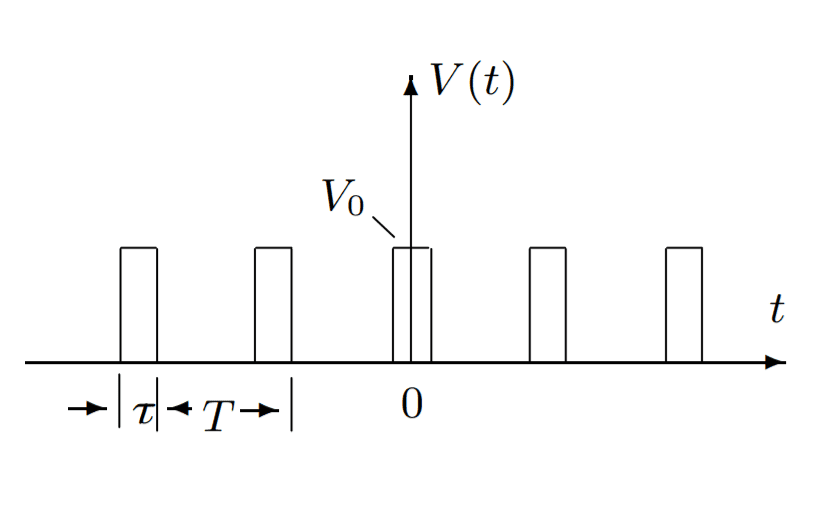
\includegraphics[width=0.9\linewidth]{pictures/sp1.png}}
        \caption{Прямоугольные импульсы}
        \label{pic:1}
    \end{minipage}
    \begin{minipage}[h]{0.5\linewidth}
        \center{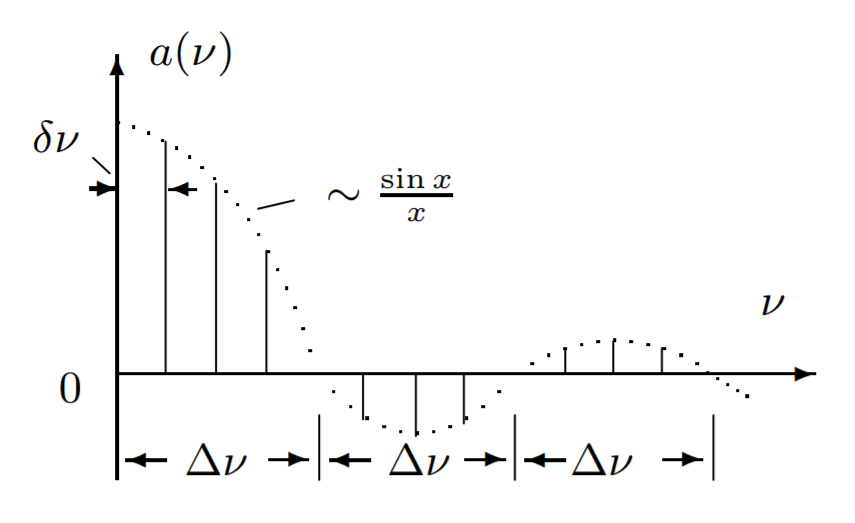
\includegraphics[width=0.9\linewidth]{pictures/sp2.png}}
        \caption{Спектр последовательности прямоугольных импульсов}
        \label{pic:2}
    \end{minipage}
\end{figure}

Назовем \textit{шириной спектра} $\Delta \omega$ расстояние от главного максимума ($\omega =0$) до первого нуля огибающей, возникающего при $n=\dfrac{2\pi}{\tau \Omega_{1}}$. При этом 

\begin{equation*}
    \Delta \omega \tau \backsimeq 2 \pi
\end{equation*}

или

\begin{equation}\label{eq:5}
	\Delta \nu \Delta t \backsimeq 1
\end{equation}

Полученное соотношение взаимной связи интервалов $\Delta \nu$ и $\Delta t$ является частным случаем соотношения неопределенности в квантовой механике.

\begin{enumerate}[resume]
	\item \textbf{Периодическая последовательность цугов} гармонического колебания $V_{0}\cos(\omega_{0}t)$ с длительностью цуга $\tau$ и периодом повторения $T$ (рис. \ref{pic:3}).
\end{enumerate}

Функция $f(t)$ снова является четной относительно $t=0$. Коэффициент при $n$-й гармонике равен

\begin{equation}\label{eq:6}
    a_{n}=\dfrac{2}{T}\int\limits_{-\frac{\tau}{2}}^{\frac{\tau}{2}}V_{0}\cos(\omega_{0}t)\cos(n \Omega_{1} t)dt=V_{0}\dfrac{\tau}{T} \bigg(\dfrac{\sin[(\omega_{0}-n\Omega_{1})\frac{\tau}{2}]}{(\omega_{0}-n\Omega_{1})\frac{\tau}{2}}+\dfrac{\sin[(\omega_{0}+n\Omega_{1})\frac{\tau}{2}]}{(\omega_{0}+n\Omega_{1})\frac{\tau}{2}} \bigg)
\end{equation}

Зависимость для случая, когда $\frac{T}{\tau}$ равно целому числу, представлена на рис. \ref{pic:4}. Сравнивая спектр последовательности прямоугольных импульсов и цугов мы видим, что они аналогичны, но их максимумы сдвинуты по частоте на величину $\omega_{0}$.

\begin{figure}[h]
    \begin{minipage}[h]{0.5\linewidth}
        \center{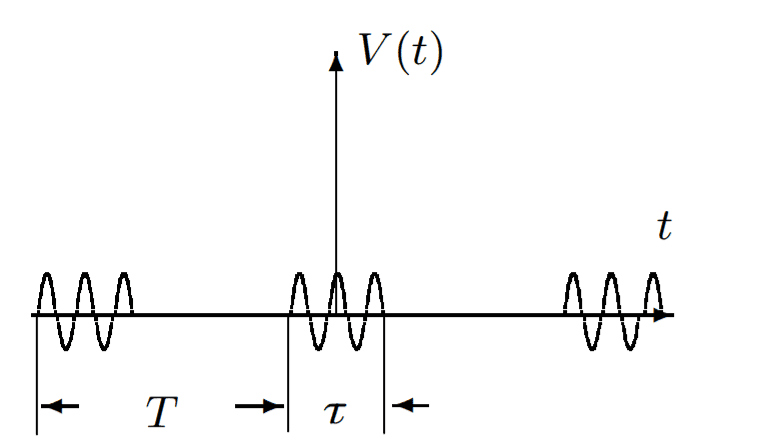
\includegraphics[width=0.9\linewidth]{pictures/sp3.png}}
        \caption{Последовательность цугов}
        \label{pic:3}
    \end{minipage}
    \begin{minipage}[h]{0.5\linewidth}
        \center{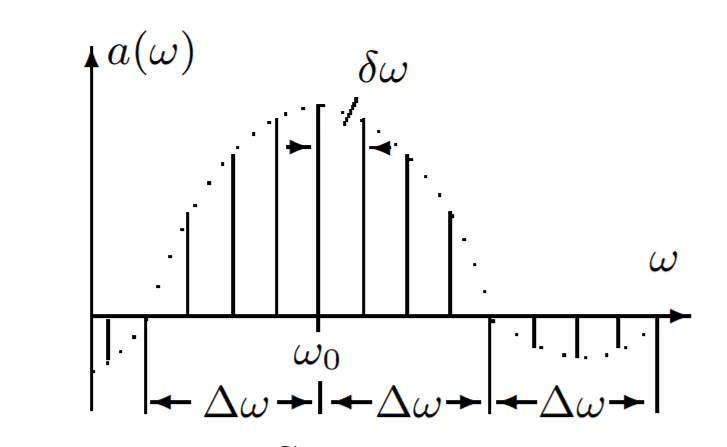
\includegraphics[width=0.9\linewidth]{pictures/sp4.png}}
        \caption{Спектр последовательности цугов}
        \label{pic:4}
    \end{minipage}
\end{figure}

\begin{enumerate}[resume]
    \item \textbf{Амплитудно-модулированные колебания.} Рассмотрим гармонические колебания высокой частоты $\omega_{0}$ , амплитуда которых медленно меняется по гармоническому закону с частотой $\Omega$ ($\Omega \ll \omega_{0})$) (рис. \ref{pic:5}):
\end{enumerate}


\begin{equation}\label{eq:7}
    f(t)=A_{0}[1+m\cos\Omega t]\cos \omega_{0}t
\end{equation}

Коэффициент $m$ называют \textbf{глубиной модуляции}. При $m<1$ амплитуда колебаний меняется от минимальной $A_{min}=A_{0}(1-m)$ до максимальной $A_{max}=A_{0}(1+m).$ Глубина модуляции может быть представлена в виде

\begin{equation}\label{eq:8}
	 m=\dfrac{A_{max}-A_{min}}{A_{max}+A_{min}}
\end{equation}

Простым тригонометрическим преобразованием можно найти спектр амплитудно - модулированных колебаний: \\

\begin{equation}\label{a}
	f(t)=A_{0}\cos(\omega_{0} t)+\dfrac{A_{0}m}{2}\cos(\omega_{0}+\Omega)t+\dfrac{A_{0}m}{2}\cos(\omega_{0}-\Omega)t.
\end{equation}


\begin{figure}[h]
    \begin{minipage}[h]{0.5\linewidth}
        \center{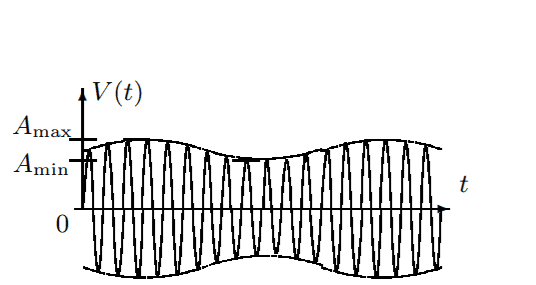
\includegraphics[width=0.9\linewidth]{pictures/sp5.png}}
        \caption{Модулированные гармонические колебания}
        \label{pic:5}
    \end{minipage}
    \begin{minipage}[h]{0.5\linewidth}
        \center{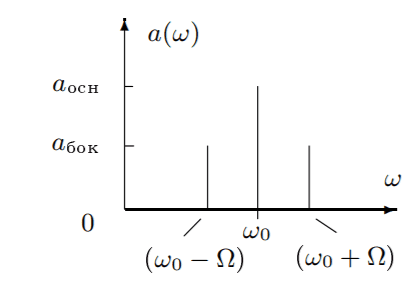
\includegraphics[width=0.9\linewidth]{pictures/sp6.png}}
        \caption{Спектр модулированных гармонических колебаний}
        \label{pic:6}
    \end{minipage}
\end{figure}

Спектр таких колебаний содержит три составляющих  основную компоненту и две боковых (рис. 6). Первое слагаемое в правой части представляет собой исходное немодулированное колебание с основной (несущей) частотой $\omega_{0}$ и амплитудой $a_{осн} = A_{0}$ . Второе и третье слагаемые соответствуют новым гармоническим колебаниям с частотами $\omega_{0} + \Omega$ и $\omega_{0} - \Omega$. Амплитуды этих двух колебаний одинаковы и составляют $\dfrac{m}{2}$ от амплитуды немодулированного колебания: $a_{бок} = \dfrac{A_{0}m}{2}$. Начальные фазы всех трех колебаний одинаковы.

\section{Экспериментальная установка}


В работе изучаются спектры периодических электрических сигналов различной формы (последовательности прямоугольных импульсов и цугов, а также амплитудно- и фазо-модулированных гармонических колебаний). Спектры этих сигналов наблюдаются с помощью спектроанализатора, входящего в состав USB-осциллографа и сравниваются с рассчитанными теоретически. Схема установки изображена на рис. \ref{pic:ustan}

\begin{figure}[h]
    \centering
    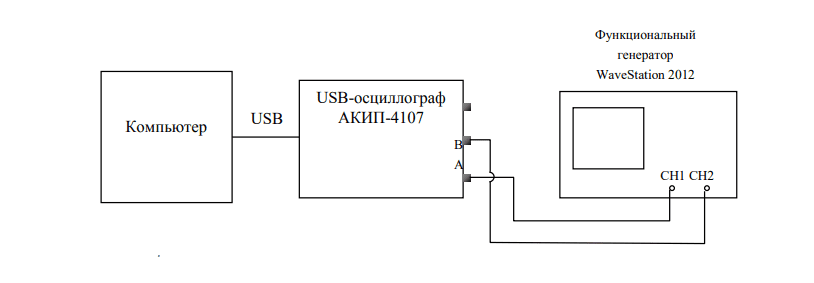
\includegraphics[width=1\linewidth]{pictures/ustan.png}
    \caption{Схема экспериментальной установки}
    \label{pic:ustan}
\end{figure}

Функциональный генератор WaveStation 2012 позволяет сформировать два различных электрических сигнала, которые выводятся на два независимых канала – "CH1" и "CH2". Сигнал с канала "CH1" подается на вход "А", а сигнал с канала "CH2" – на вход "В" USB-осциллографа. Затем эти сигналы подаются на вход компьютера через USB-соединение. При работе USB-осциллографа в режиме осциллографа, на экране компьютера можно наблюдать каждый из сигналов в отдельности, а также их произведение. В режиме спектроанализатора можно наблюдать спектры этих сигналов. При включении функционального генератора, на его экране отображается информация о параметрах электрического сигнала. На рис.\ref{pic:gen-1} показаны области на экране генератора, в которых отображены следующие 
данные:

А – форма или тип сигнала и номер выходного канала;
Б – форма и параметры выходного сигнала;
В – область установки параметров выходного сигнала;
Г – форма или тип сигнала;
Д – экранное меню для установки параметров сигнала.

\begin{figure}[h]
    \centering
    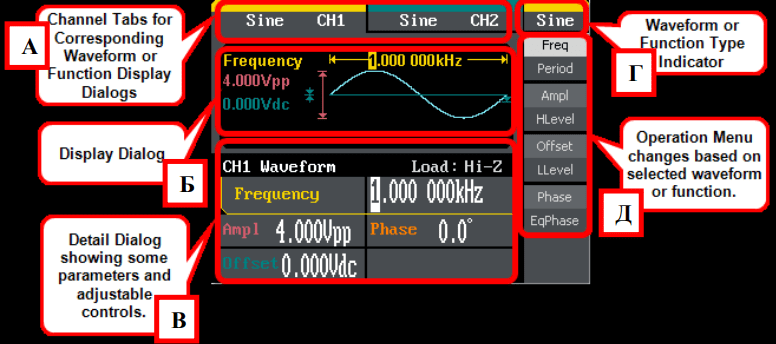
\includegraphics[width=0.8\linewidth]{pictures/generator1.png}
    \caption{Экран генератора}
    \label{pic:gen-1}
\end{figure}

Передняя панель функционального генератора показана на рис.\ref{pic:gen-2}. 1 – кнопка включения; 2 – USB-разъем; 3 – экран; 4 – кнопки экранного меню; 5 – кнопки выбора типа сигналов; 6 – цифровая панель; 7 - функциональные кнопки; 8 – разъемы с кнопками включения (выключения) выходных сигналов 1-го и 2-го каналов; 9 – кнопки перемещения; 10 – подстроечный регулятор.

\begin{figure}[h]
    \centering
    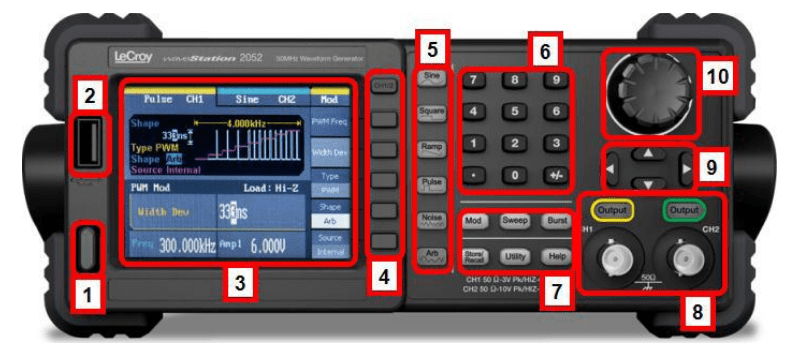
\includegraphics[width=0.9\linewidth]{pictures/generator2.png}
    \caption{Передняя панель функционального генератора}
    \label{pic:gen-2}
\end{figure}

\FloatBarrier

\section{Результаты измерений и обработка данных}

\begin{enumerate}
    \item Ознакомимся с устройством панелей приборов. Изучим расположение основных кнопок и ручек настройки.
    \item Подключим выход генератора к каналу осциллографа и включим приборы в сеть.
\end{enumerate}

\subsection*{А. Исследование спектра периодической последовательности прямоугольных импульсов и проверка соотношений неопределённостей}

\begin{enumerate}[resume]
    \item Настроим генерацию прямоугольных импульсов. Частота повторения $\nu_\text{повт} = 1$ кГц (период $T = 1 /\nu_\text{повт} = 1$ мс) и длительность импульса $\tau = T/20 = 50$ мкс.
    \item Получим устойчивую картину сигналов на экране осциллографа.
    \item Получим на экране спектр сигнала. 
    \item Изменяя на генераторе параметры сигнала, пронаблюдаем как изменяется спектр при изменении параметров сигнала. Спектры представлены на рис. \ref{pic:spectr-1}, \ref{pic:spectr-2}, \ref{pic:spectr-3}
\end{enumerate}

Как видно при увеличении частоты спектр растягивается по горизонтали.

При увеличении периода повторения спектр растягивается по вертикали.

\begin{figure}[!ht]
        \centering
	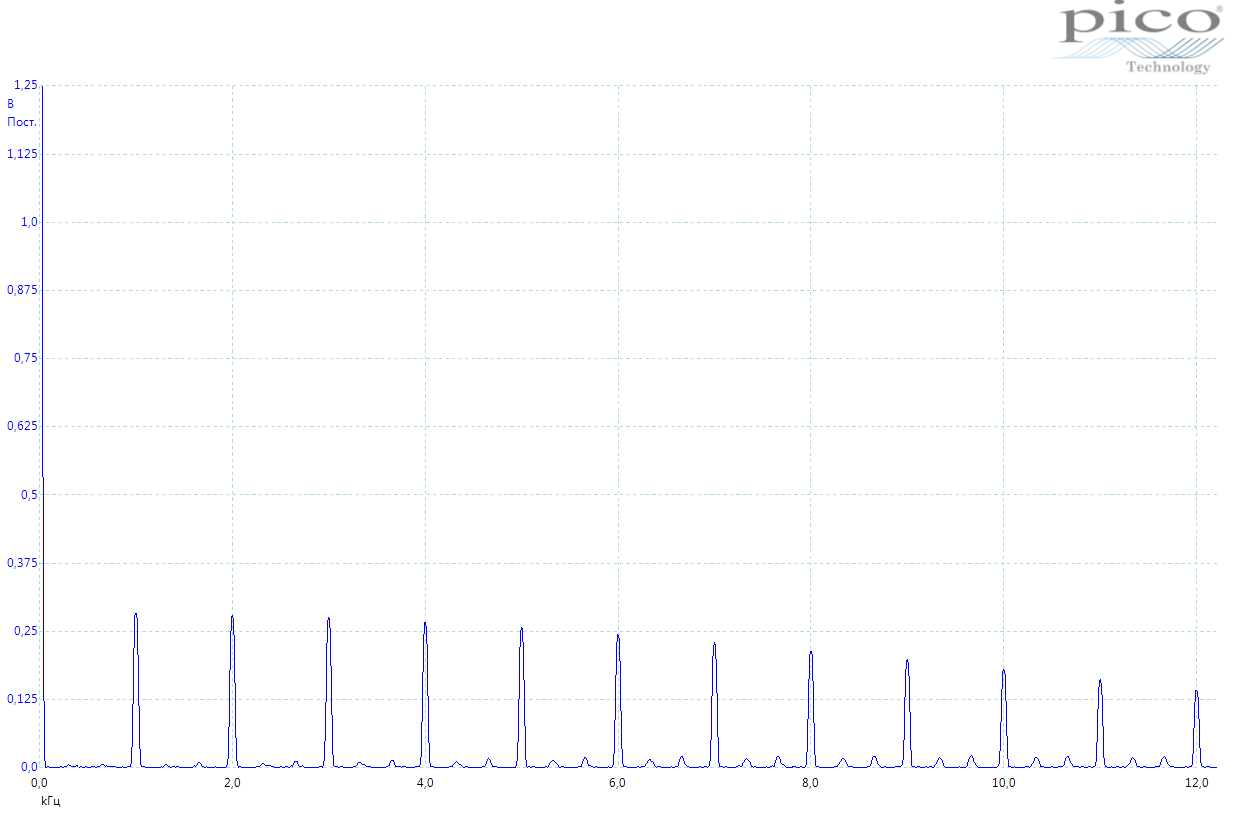
\includegraphics[width=0.9\textwidth]{pictures/6/a_0_1_50.png}
	\caption{\textit{Спектр сигнала при $\nu_\text{повт} = 1$ кГц, $\tau = 50$ мкс}}
	\label{pic:spectr-1}
\end{figure}

\begin{figure}[!ht]
        \centering
	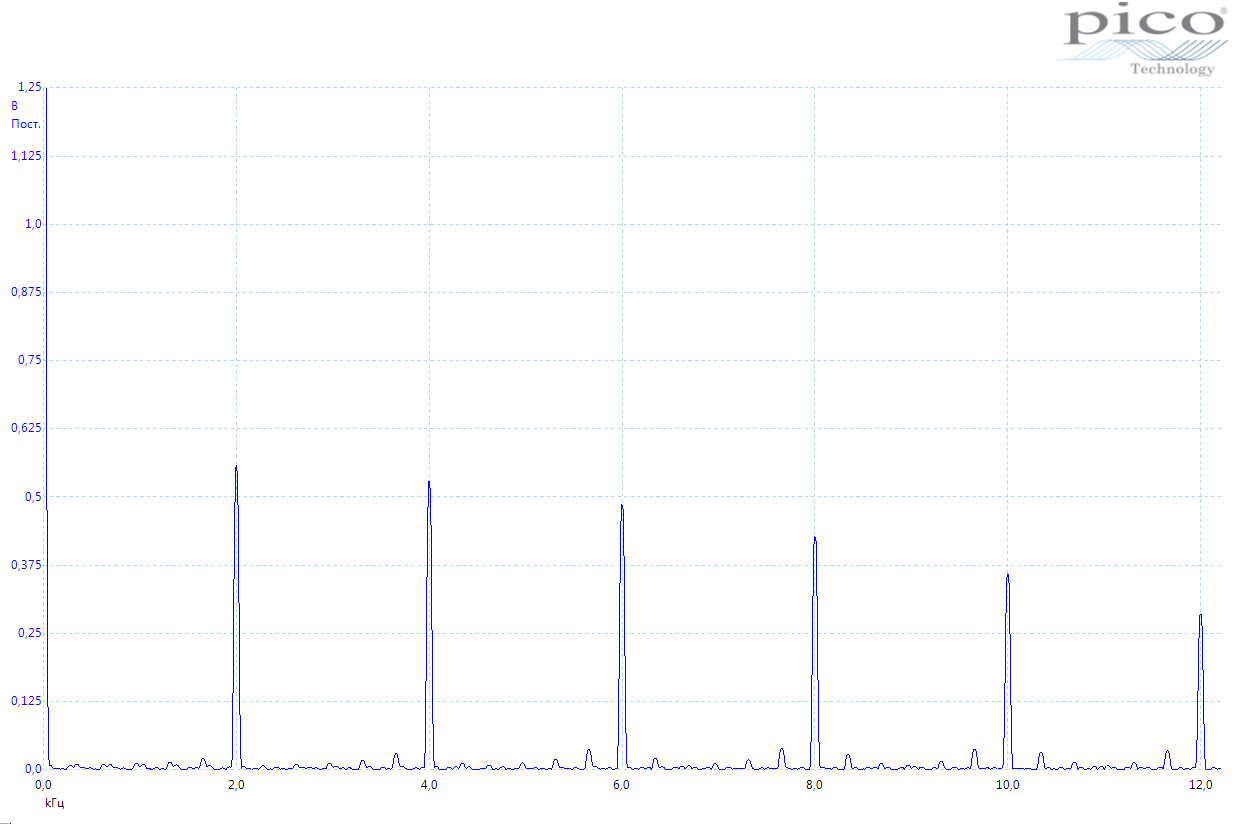
\includegraphics[width=0.9\textwidth]{pictures/6/a_2_50.png}
	\caption{\textit{Спектр сигнала при $\nu_\text{повт} = 2$ кГц, $\tau = 50$ мкс}}
	\label{pic:spectr-2}
\end{figure}

\begin{figure}[h]
        \centering
	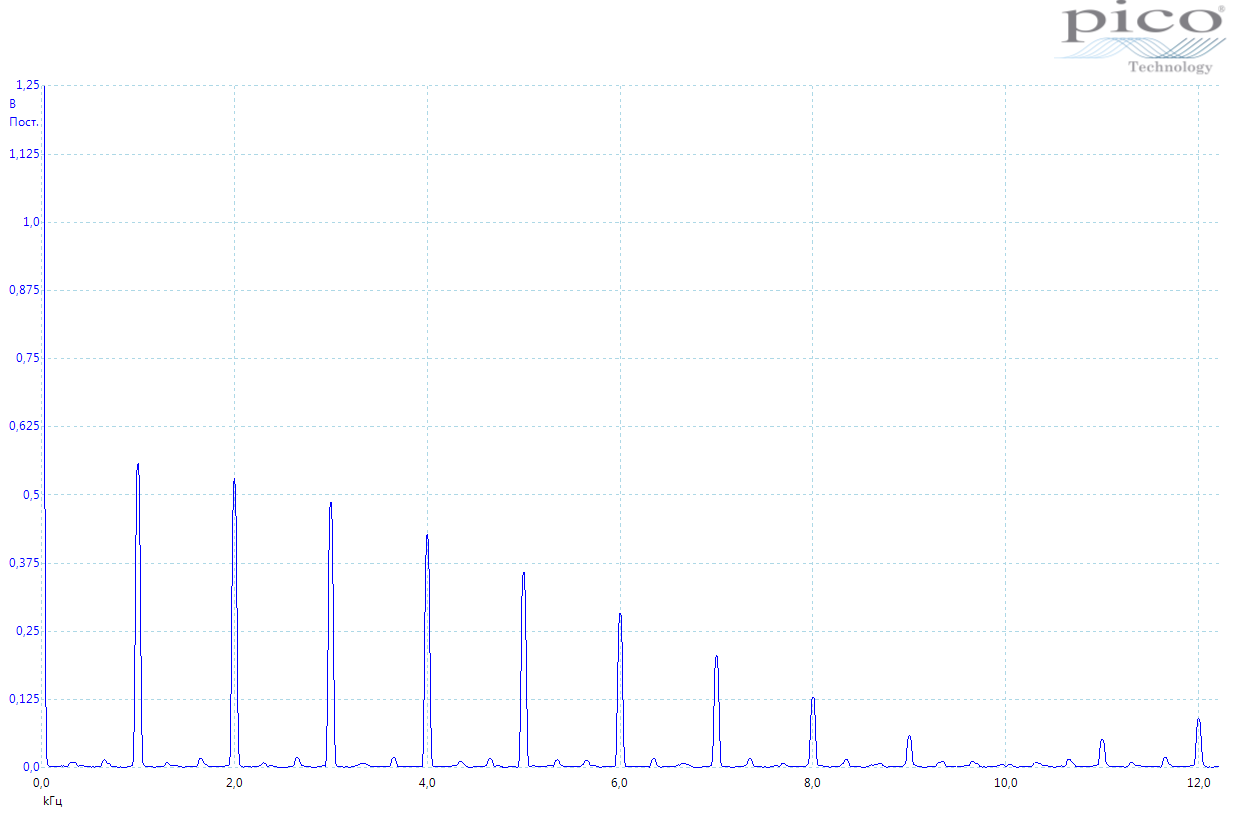
\includegraphics[width=0.9\textwidth]{pictures/6/a_1_100.png}
	\caption{\textit{Спектр сигнала при $\nu_\text{повт} = 1$ кГц, $\tau = 100$ мкс}}
	\label{pic:spectr-3}
\end{figure}

\FloatBarrier

\begin{enumerate}[resume]
    \item При фиксированных параметрах $\nu_\text{повт} = 1$ кГц, $\tau = 50$ мкс измерим частоты и амплитуды нескольких спектральных компонент. Результаты измерений занесем в таблицу \ref{table:1}
\end{enumerate}

\begin{table}[!ht]
    \centering
    \caption{\textit{Измерение амплитуды и частоты гармоник спектра}}
    \begin{tabular}{|l|l|l|l|l|}
        \hline
        $n$ & $a_n$, кГц & $a_n/a_1$ & $\nu_n$, мВ \\ \hline
        1 & 1,001     & 1,0       & 277,6  \\ \hline
        2 & 2,003     & 2,0       & 276,0  \\ \hline
        3 & 2,995     & 3,0       & 269,8  \\ \hline
        4 & 4,008     & 4,0       & 260,4  \\ \hline
        5 & 5,000     & 5,0       & 254,1  \\ \hline
        6 & 6,002     & 6,0       & 243,1  \\ \hline
        7 & 7,004     & 7,0       & 225,8  \\ \hline
        8 & 7,996     & 8,0       & 211,7  \\ \hline                 
    \end{tabular}
    \label{table:1}
\end{table}

Как видно, частота гармоники совпадает с $\nu_\text{повт}$, а остальные гармоники кратны первой. Значит экспериментально теоретическая зависимость выполняется.

\begin{enumerate}[resume]
    \item Измерим зависимость полной ширины спектра $\Delta \nu$ от длительности импульса при фиксированном периоде повторения. Результаты измерений запишем в таблицу \ref{table:2}.
\end{enumerate}

\begin{table}[!ht]
    \centering
    \caption{\textit{Зависимость ширины спектра от длительности импульса}}
    \begin{tabular}{|l|l|l|l|l|l|l|l|l|l|l|l|}
        \hline
        $\tau$, мкс       & 20    & 38    & 56    & 74    & 92    & 110  & 128  & 146  & 164  & 182  & 200  \\ \hline
        $\Delta \nu$, кГц & 46,00 & 25,00 & 17,33 & 13,36 & 11,11 & 9,01 & 8,00 & 7,00 & 6,03 & 5,53 & 4,98 \\ \hline
        $n$               & 1     & 2     & 3     & 4     & 5     & 6    & 7    & 8    & 9    & 10   & 11   \\ \hline
    \end{tabular}
    \label{table:2}
\end{table}

\begin{enumerate}[resume]
    \item Измерим зависимость расстояния между гармониками $\delta \nu$ спектра от периода повторения $T$ при $\tau = 100$ мкс. Результаты измерений запишем в таблицу \ref{table:3}.
\end{enumerate}

\begin{table}[!ht]
    \centering
    \caption{\textit{Зависимость расстояния между гармониками от периода повторения}}
    \begin{tabular}{|l|l|l|l|l|}
        \hline
        $n$ & $T$, мс & $\nu$, кГц & $T / \tau$ & $\delta \nu$, кГц \\ \hline
        1 & 0,2 & 5,000 & 2 & 5,007 \\ \hline
        2 & 0,800 & 0,125 & 8 & 1,252 \\ \hline
        3 & 1,400 & 0,071 & 14 & 0,715 \\ \hline
        4 & 2,000 & 0,050 & 20 & 0,501 \\ \hline
        5 & 2,600 & 0,038 & 26 & 0,385 \\ \hline
        6 & 3,200 & 0,031 & 32 & 0,313 \\ \hline
        7 & 3,800 & 0,026 & 38 & 0,264 \\ \hline
        8 & 4,400 & 0,023 & 44 & 0,226 \\ \hline
        9 & 5,000 & 0,020 & 50 & 0,203 \\ \hline
    \end{tabular}
    \label{table:3}
\end{table}

\begin{enumerate}[resume]
    \item Построим графики зависимостей $\Delta \nu (1 / \tau)$ и $\delta \nu (1 / T)$. Зависимость должна получиться линейная. Графики изобразим на рис. \ref{graph:1} и \ref{graph:2} соответственно.
\end{enumerate}

\begin{figure}[!ht]
        \centering
	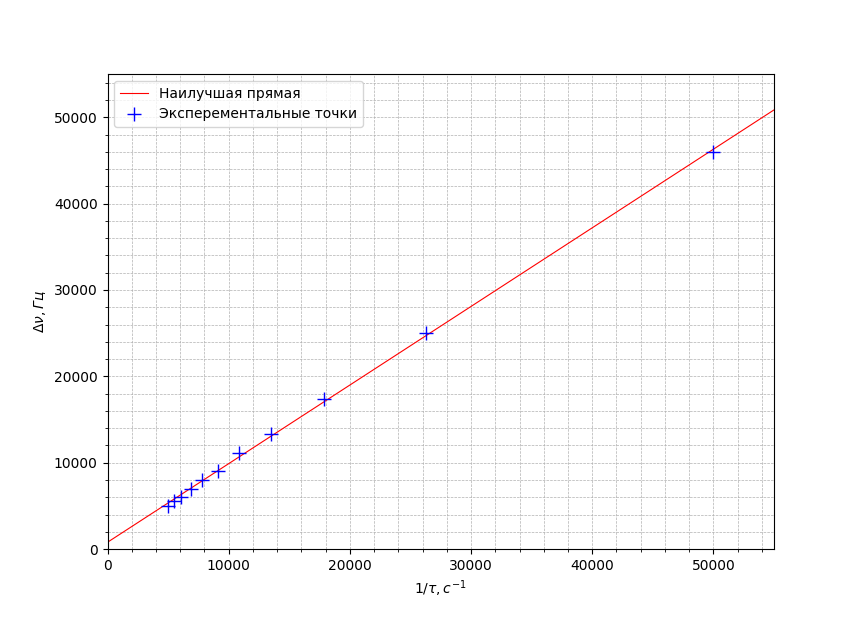
\includegraphics[width=1.0\textwidth]{pictures/10/Deltanu-tau.png}
	\caption{\textit{Зависимость $\Delta \nu (1 / \tau)$}}
	\label{graph:1}
\end{figure}

\begin{figure}[!ht]
        \centering
	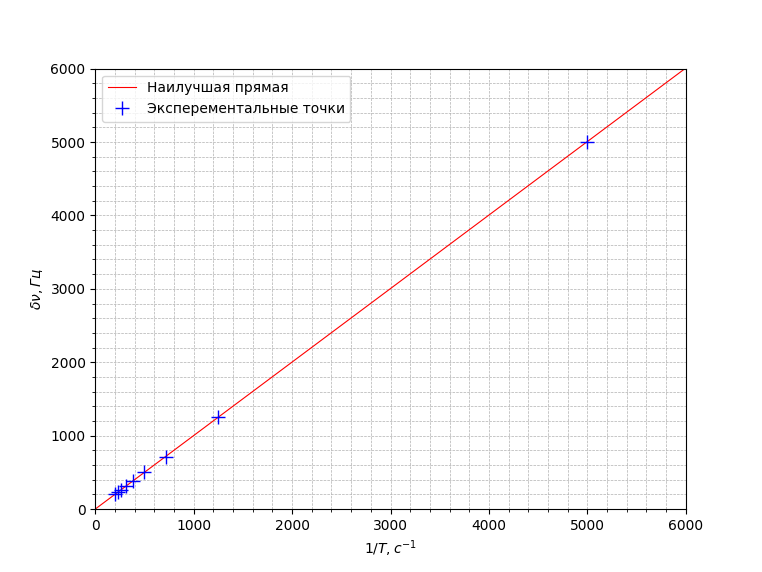
\includegraphics[width=1.0\textwidth]{pictures/10/deltanu-T.png}
	\caption{\textit{Зависимость $\delta \nu (1 / T)$}}
	\label{graph:2}
\end{figure}

\FloatBarrier

\subsection*{Б. Наблюдение спектра периодической последовательности цугов}

\begin{enumerate}[resume]
    \item Установим генератор в режим подачи синусоидальных сигналов с частотой $\nu_0 = 50$ кГц, период повторения $T = 1$ мс, число периодов синусоиды $N = 5$. Получим устойчивую картину сигнала.
    \item Получим спектр сигнала на экране.
    \item Изменяя параметры $\nu_0$, $T$, $N$ пронаблюдаем как изменяется вид спектра. Спектры изображены на рис. \ref{pic:zug-1}, \ref{pic:zug-2}, \ref{pic:zug-3}.
\end{enumerate}


\FloatBarrier

\begin{figure}[!ht]
        \centering
	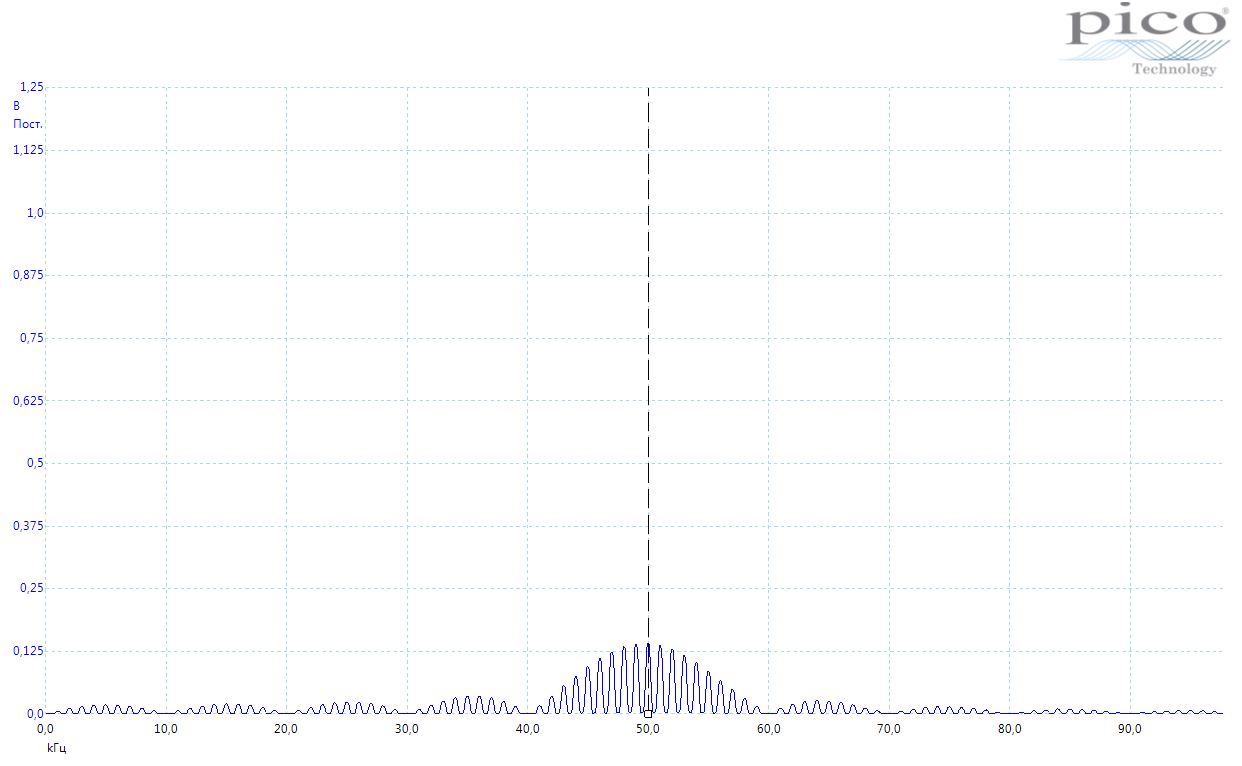
\includegraphics[width=0.9\textwidth]{pictures/13/50_1_5.png}
	\caption{\textit{Спектр сигнала при $\nu_\text{повт} = 50$ кГц, $T = 1$ мс, $N = 5$}}
	\label{pic:zug-1}
\end{figure}

\begin{figure}[!ht]
        \centering
	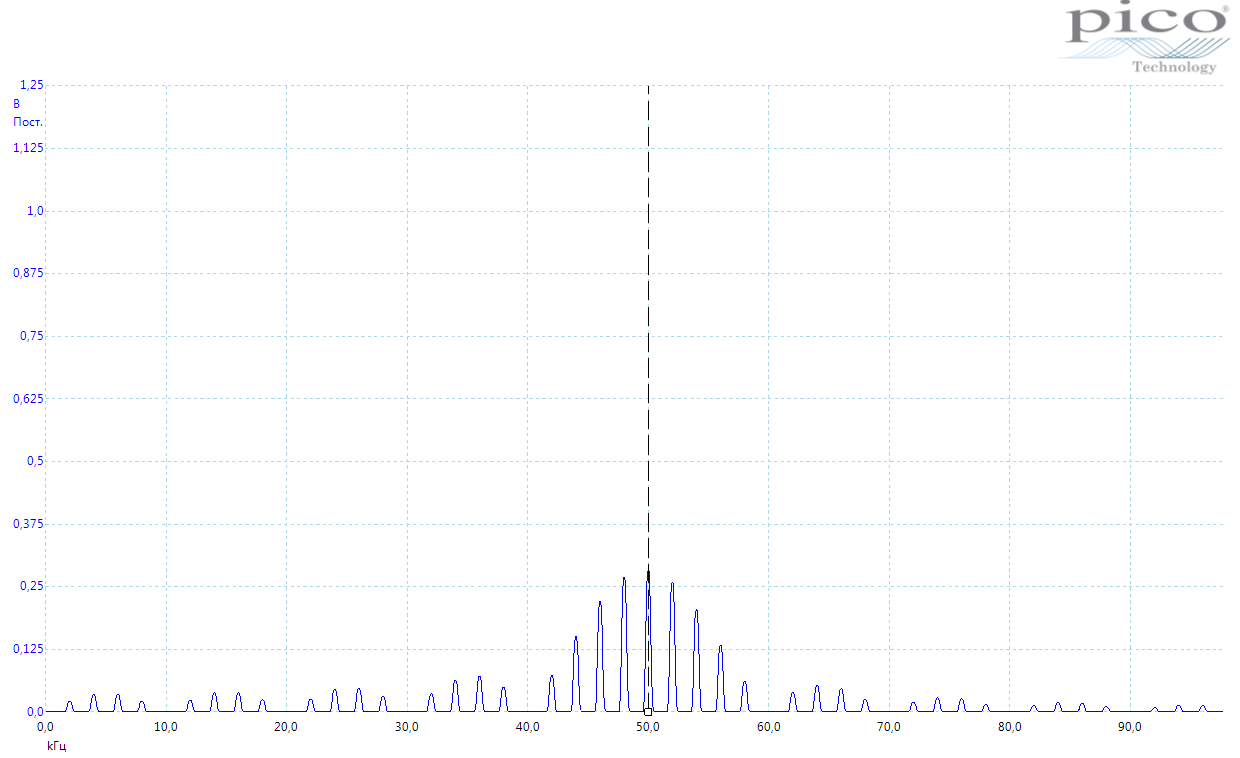
\includegraphics[width=0.9\textwidth]{pictures/13/50_0.5_5.png}
	\caption{\textit{Спектр сигнала при $\nu_\text{повт} = 50$ кГц, $T = 0,5$ мс, $N = 5$}}
	\label{pic:zug-2}
\end{figure}

\begin{figure}[!ht]
        \centering
	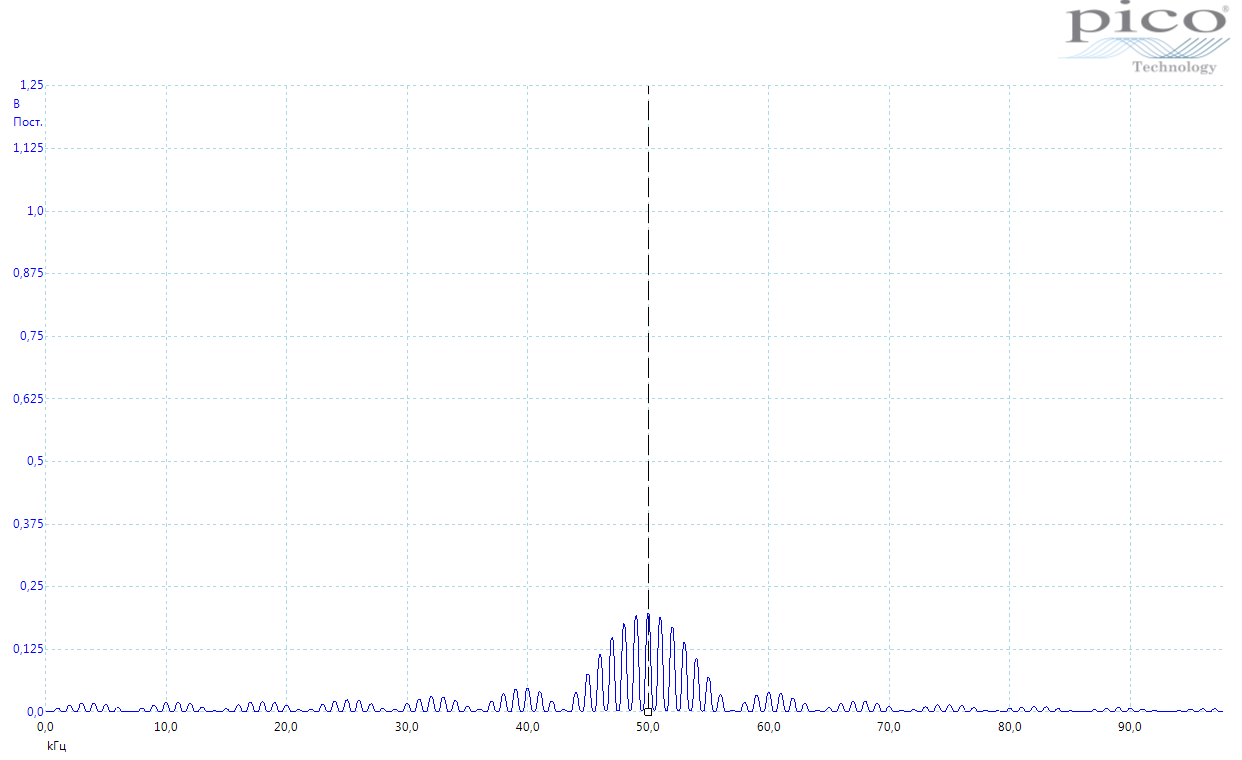
\includegraphics[width=0.9\textwidth]{pictures/13/50_1_8.png}
	\caption{\textit{Спектр сигнала при $\nu_\text{повт} = 50$ кГц, $T = 1$ мс, $N = 8$}}
	\label{pic:zug-3}
\end{figure}

\FloatBarrier

\begin{enumerate}[resume]
    \item При этих параметрах сигнала измерим положение центра спектра, его ширину и расстояние между гармониками. Результаты измерений запишем в таблицу \ref{table:4}.
\end{enumerate}

\FloatBarrier
\begin{table}[]
    \centering
    \caption{\textit{Измеренные характеристики спектра для разных параметров}}
    \begin{tabular}{|l|l|l|l|l|}
        \hline
        спектр & $a_c$, мВ & $\Delta \nu$, кГц & $\delta \nu$, кГц & $\delta \nu \cdot T$ \\ \hline
        рис. \ref{pic:zug-1} & 139,6 & 9,961 & 1,008 & 1,008 \\ \hline
        рис. \ref{pic:zug-2} & 277,6 & 9,961 & 2,004 & 1,002 \\ \hline
        рис. \ref{pic:zug-3} & 224,3 & 5,912 & 1,004 & 1,004 \\ \hline
    \end{tabular}
    \label{table:4}
\end{table}
\FloatBarrier

Убедимся в справедливости теоремы смещения и соотношений неопределенностей.

\begin{equation*}
    \Delta \omega \cdot \Delta t \sim 2 \pi \implies 2 \pi \delta \nu \cdot T \sim 2 \pi
\end{equation*}
\begin{equation*}
    \delta \nu \cdot T \sim 1
\end{equation*}

Посчитаем и занесем в таблицу \ref{table:4}. Как видно соотношение неопределенности выполняется.

\subsection{В. Наблюдение спектра периодической последовательности гауссианов}

Данный раздел работы не выполнялся.

\subsection{Г. Исследование спектра амплитудно-модулированного сигнала}

\begin{enumerate}
    \setcounter{enumi}{18}
    \item Установим на генераторе режим модулированного по амплитуде синусоидального сигнала с параметрами $\nu_0 = 50$ кГц, частота модуляции $\nu_\text{мод} = 2$ кГц, глубина модуляции 50\% ($m = 0,5$). Получим на экране осциллографа устойчивую картину сигнала.
    \item Измерим максимальную и минимальную амплитуды сигнала: $A_\text{max} = 1,232$ В, $A_\text{min} = 0,4256$ В.
\end{enumerate}

\begin{equation}
    \frac{A_\text{max} - A_\text{min}}{A_\text{max} + A_\text{min}} = 0,49 \approx = m
\end{equation}

Как видно равенство выполняется.

\begin{enumerate}[resume]
    \item получим на экране спектр сигнала. Посмотрим как меняется спектр при изменении частоты модуляции. Спектры приведены на рис. \ref{pic:mod-1} и \ref{pic:mod-2}
\end{enumerate}

\FloatBarrier
\begin{figure}[!ht]
        \centering
	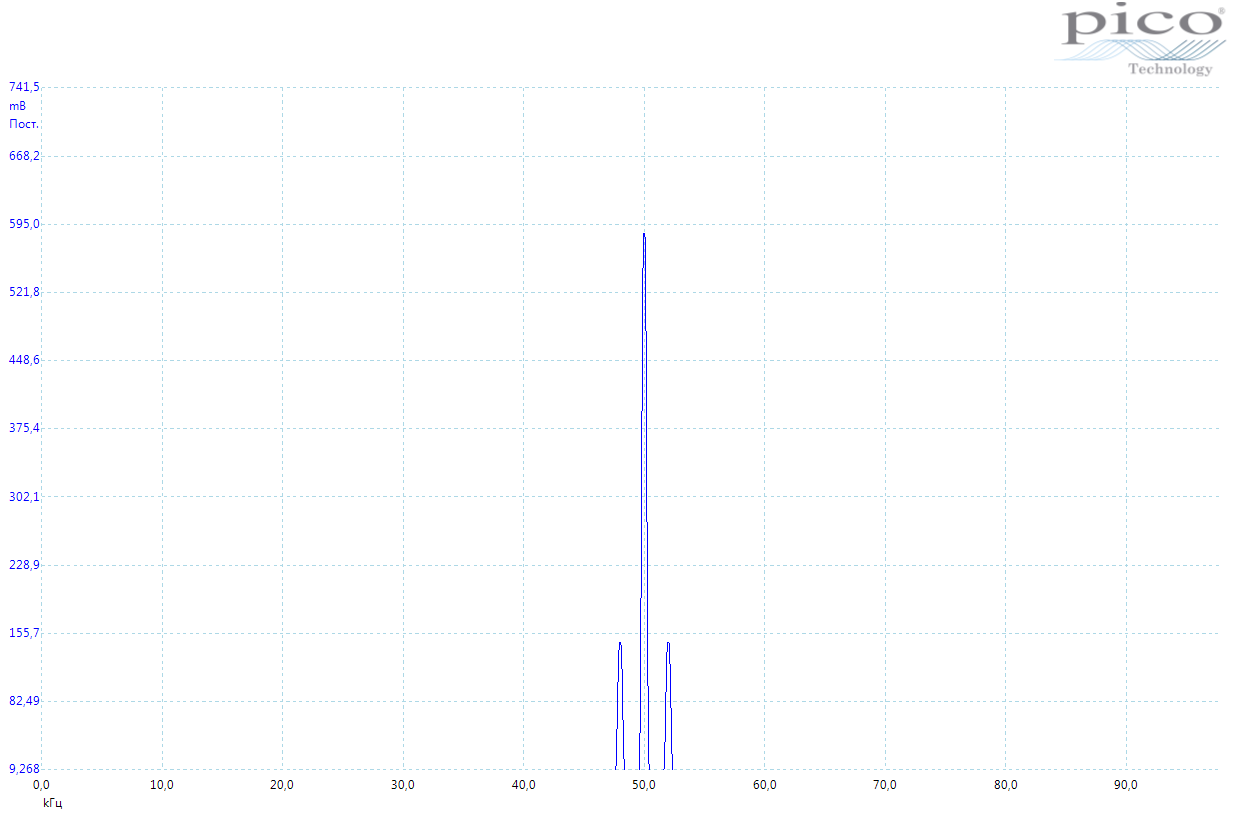
\includegraphics[width=0.9\textwidth]{pictures/21/50_2.png}
	\caption{\textit{Спектр сигнала при $\nu_0 = 50$ кГц, $\nu_\text{мод} = 2$ кГц}}
	\label{pic:mod-1}
\end{figure}

\begin{figure}[!ht]
        \centering
	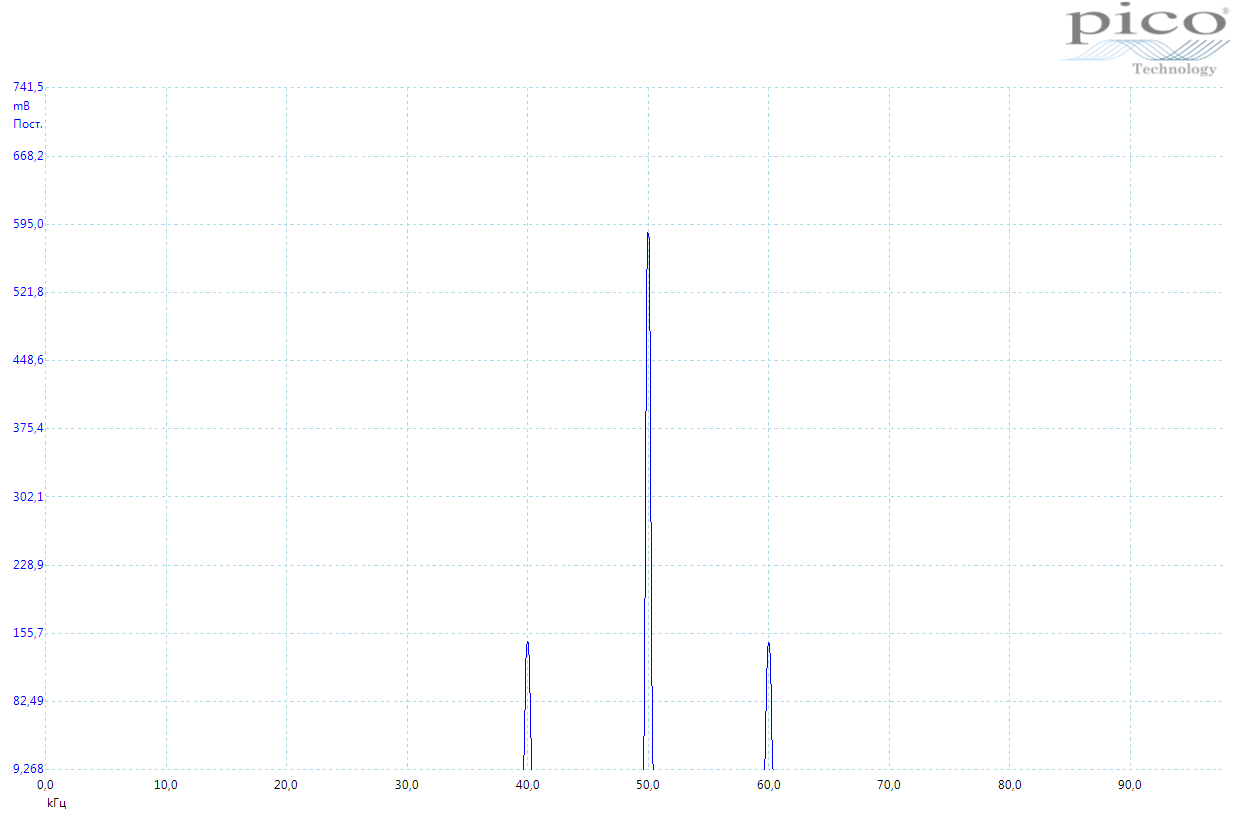
\includegraphics[width=0.9\textwidth]{pictures/21/50_10.png}
	\caption{\textit{Спектр сигнала при $\nu_0 = 50$ кГц, $\nu_\text{мод} = 10$ кГц}}
	\label{pic:mod-2}
\end{figure}

\FloatBarrier

\begin{enumerate}[resume]
    \item Изменяя глубину модуляции будем замерять амплитуды боковой и центральной гармоник. Результаты измерений запишем в таблицу \ref{table:5}.
\end{enumerate}

\FloatBarrier
\begin{table}[!ht]
    \centering
    \caption{\textit{Измерение зависимости $a_\text{бок}/a_\text{осн}$ от $m$}}
    \begin{tabular}{|l|l|l|l|l|}
        \hline
        $m$ & $m, \%$ & $a_\text{бок}$, мВ & $a_\text{осн}$, мВ & $a_\text{бок}/a_\text{осн}$ \\ \hline
        0,10 & 10    & 25,6       & 592,7      & 0,043 \\ \hline
        0,20 & 20    & 57,1       & 585,4      & 0,098 \\ \hline
        0,30 & 30    & 87,9       & 585,4      & 0,150 \\ \hline
        0,40 & 40    & 115,3      & 585,4      & 0,197 \\ \hline
        0,50 & 50    & 144,3      & 585,4      & 0,246 \\ \hline
        0,60 & 60    & 176,8      & 585,4      & 0,302 \\ \hline
        0,70 & 70    & 202,4      & 585,4      & 0,346 \\ \hline
        0,80 & 80    & 233,2      & 585,4      & 0,398 \\ \hline
        0,90 & 90    & 264,0      & 585,4      & 0,451 \\ \hline
        1,00 & 100   & 293,0      & 585,4      & 0,501 \\ \hline 
    \end{tabular}
    \label{table:5}
\end{table}
\FloatBarrier

\begin{enumerate}[resume]
    \item Построим график зависимости $a_\text{бок}/a_\text{осн}$ от $m$. Грфик изобразим на рисунке \ref{graph:3}.
\end{enumerate}

\FloatBarrier
\begin{figure}[!ht]
        \centering
	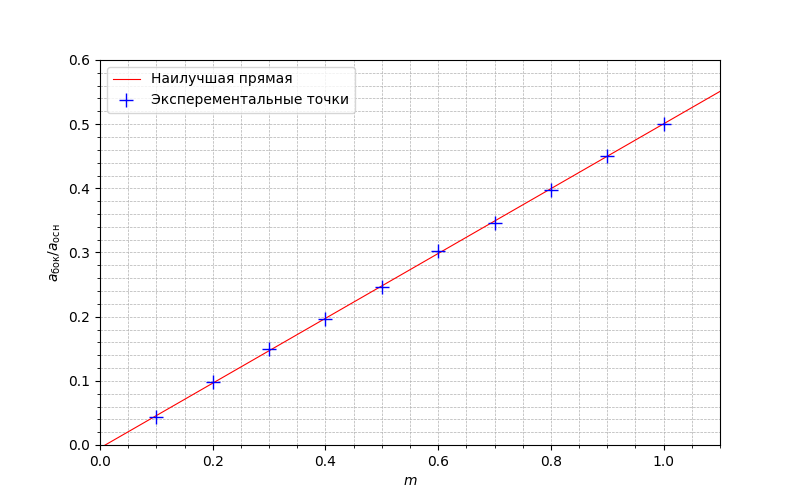
\includegraphics[width=1.0\textwidth]{pictures/graph-23.png}
	\caption{\textit{График зависимости $a_\text{бок}/a_\text{осн}$ от $m$}}
	\label{graph:3}
\end{figure}
\FloatBarrier

Как видно результат хорошо совпадает с теоретическим.

\subsection{Д. Наблюдение спектра сигнала, модулированного по фазе}

\begin{enumerate}[resume]
    \item Установим на генераторе режим модулированного по фазе сигнала с несущей $\nu_0 = 50$ кГц, частотой модуляции $\nu_\text{мод} = 2$ кГц и максимальным отклонением фазы $\phi_m = 30^\circ$. Получим на экране устойчивую картину сигнала.
    \item Получим спектр сигнала, меняя параметры пронаблюдаем как он изменяется. Спектры представлены на рис. \ref{pic:phase-1}
\end{enumerate}

\FloatBarrier
\begin{figure}[!ht]
        \centering
	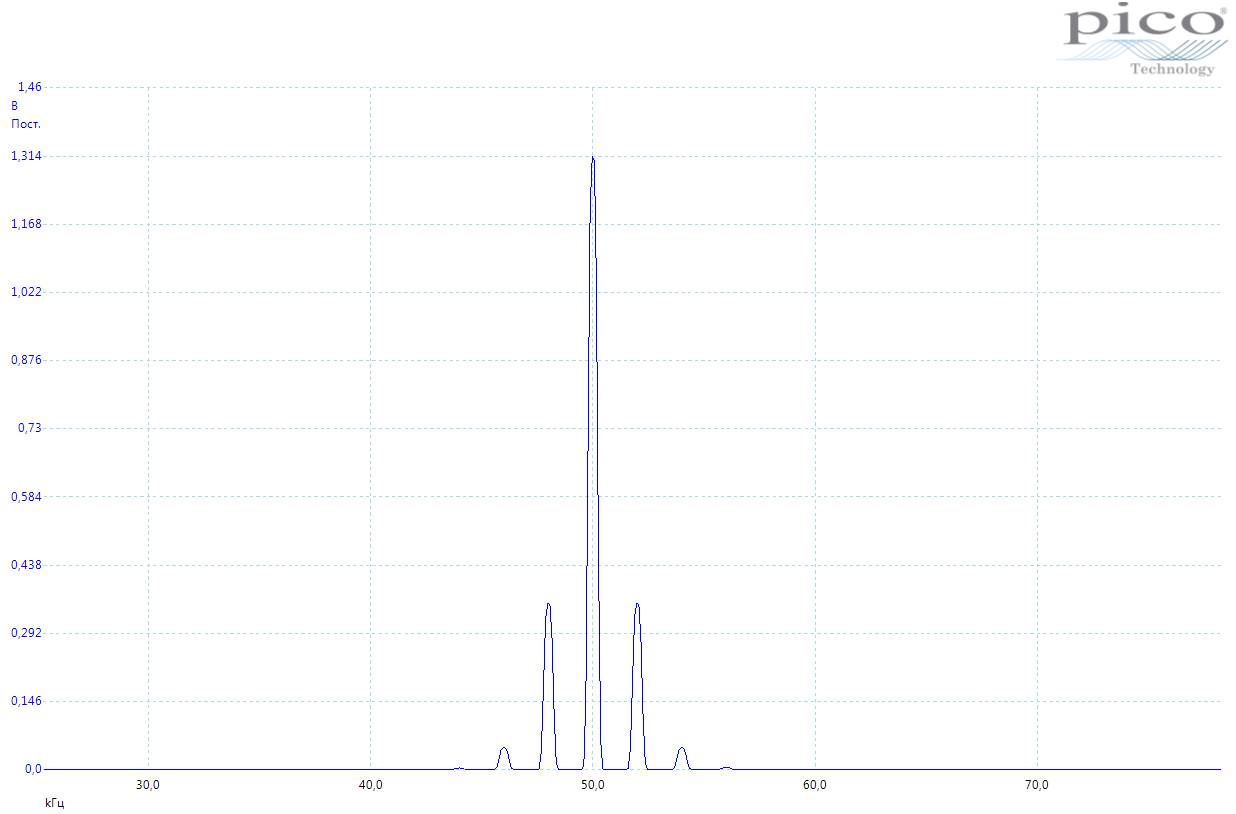
\includegraphics[width=0.9\textwidth]{pictures/25/50_2_30.png}
	\caption{\textit{Спектр сигнала при $\nu_0 = 50$ кГц, $\nu_\text{мод} = 2$ кГц, $\phi_m = 30^\circ$}}
	\label{pic:phase-1}
\end{figure}

\begin{figure}[!ht]
        \centering
	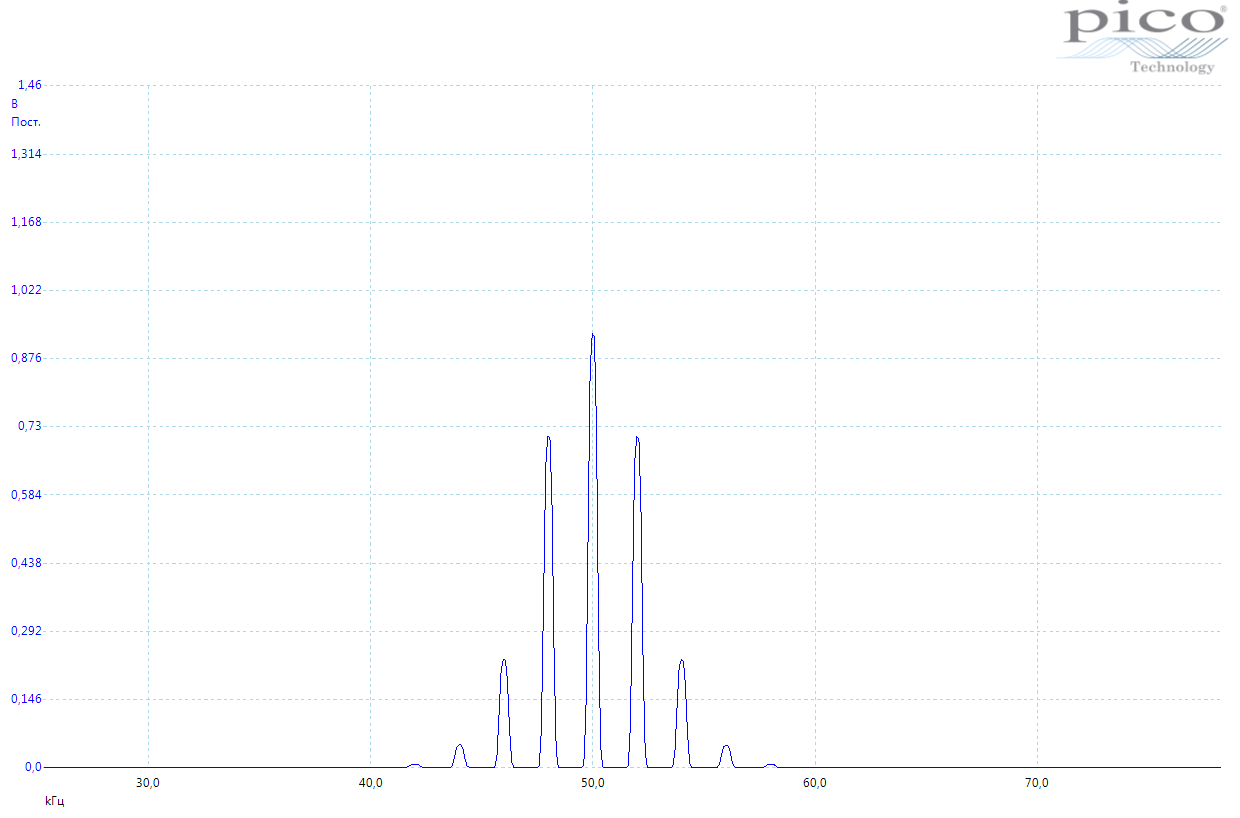
\includegraphics[width=0.9\textwidth]{pictures/25/50_2_70.png}
	\caption{\textit{Спектр сигнала при $\nu_0 = 50$ кГц, $\nu_\text{мод} = 2$ кГц, $\phi_m = 70^\circ$}}
	\label{pic:phase-2}
\end{figure}

\begin{figure}[!ht]
        \centering
	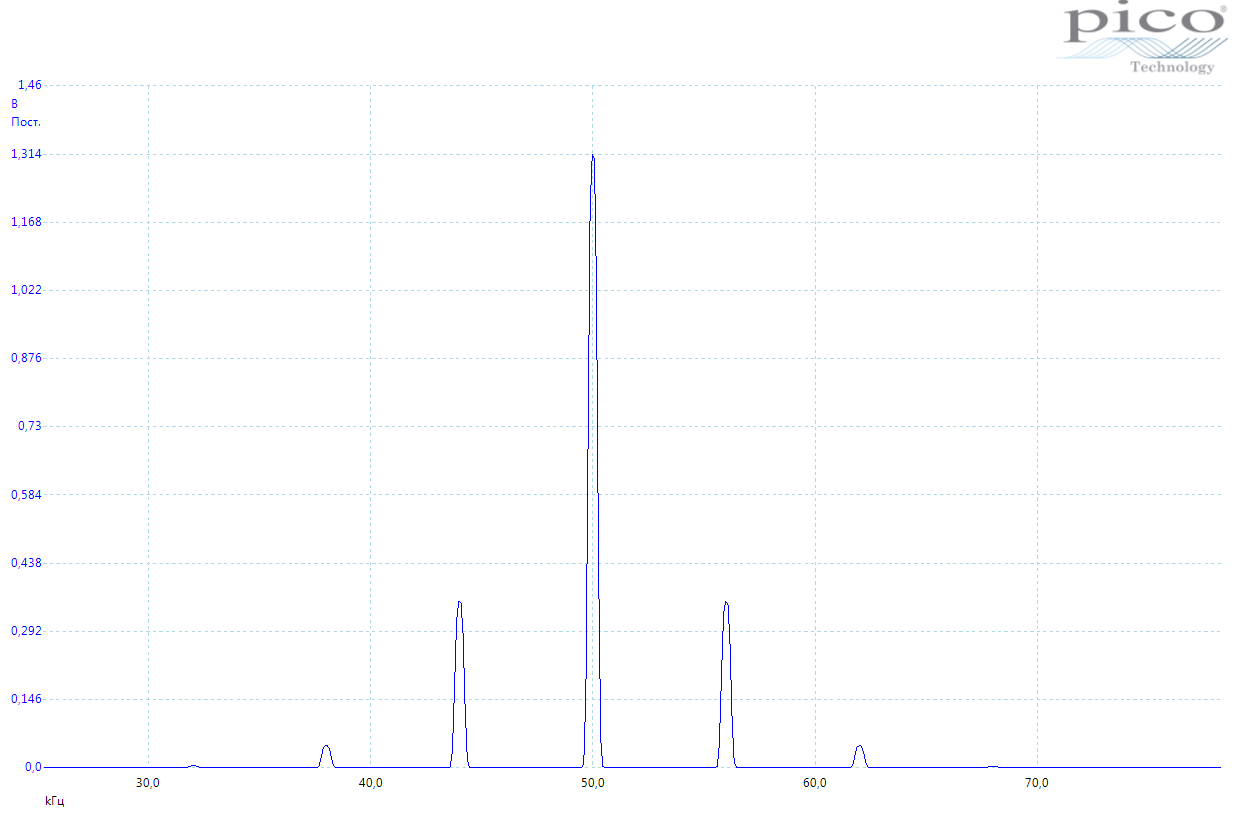
\includegraphics[width=0.9\textwidth]{pictures/25/50_6_30.png}
	\caption{\textit{Спектр сигнала при $\nu_0 = 50$ кГц, $\nu_\text{мод} = 6$ кГц, $\phi_m = 30^\circ$}}
	\label{pic:phase-3}
\end{figure}
\FloatBarrier

\subsection{Е. Изучение фильтрации сигналов}

\begin{enumerate}[resume]
    \item Для RC-цепочки рассчитаем ее характерное время и соответствующую частоту: $C = 1000$ пФ, $R = 3$ кОм.
\end{enumerate}

\begin{equation*}
    \tau_{RC} = RC \approx = 3 \ \text{мкс}
\end{equation*}
\begin{equation*}
    \nu_{RC} = 1 / \tau_{RC} \approx 333 \ \text{кГц}
\end{equation*}

Соберем схему с RC-цепочкой. Подадим на нее последовательность прямоугольных импульсов с периодом повторения $T = 3$ мкс и длительностью $\tau = 150$ нс.

\begin{enumerate}[resume]
    \item Пронаблюдаем форму сигнала и его спектр на выходе RC-цепочки для нескольких значений параметров. Сигналы представлены на рис. \ref{pic:signal-1}
\end{enumerate}

\FloatBarrier
\begin{figure}[!ht]
        \centering
	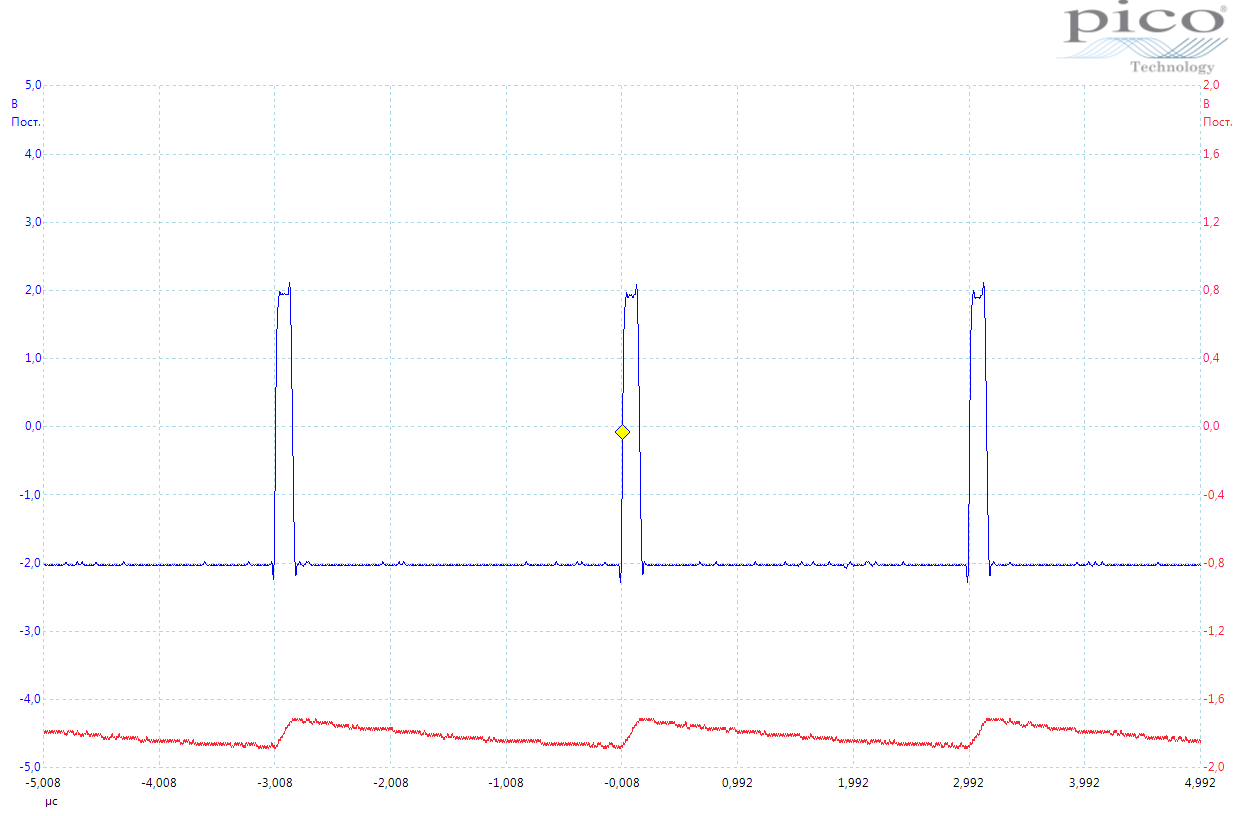
\includegraphics[width=0.9\textwidth]{pictures/27/3_150.png}
	\caption{\textit{Спектр сигнала на выходе RC-цепочки при $T = 3$ мкс, $\tau = 150$ нс}}
	\label{pic:signal-1}
\end{figure}

\begin{figure}[!ht]
        \centering
	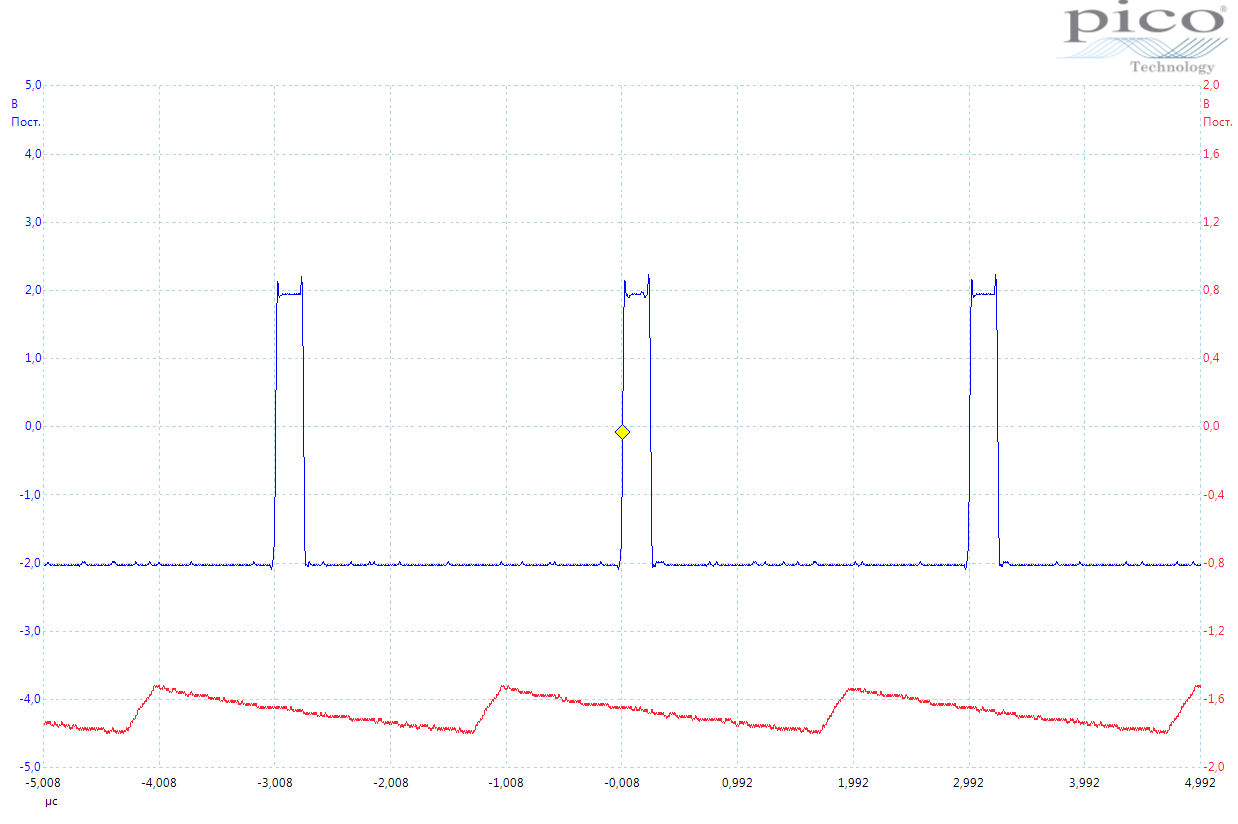
\includegraphics[width=0.9\textwidth]{pictures/27/3_250.png}
	\caption{\textit{Спектр сигнала на выходе RC-цепочки при $T = 3$ мкс, $\tau = 250$ нс}}
	\label{pic:signal-2}
\end{figure}

\begin{figure}[!ht]
        \centering
	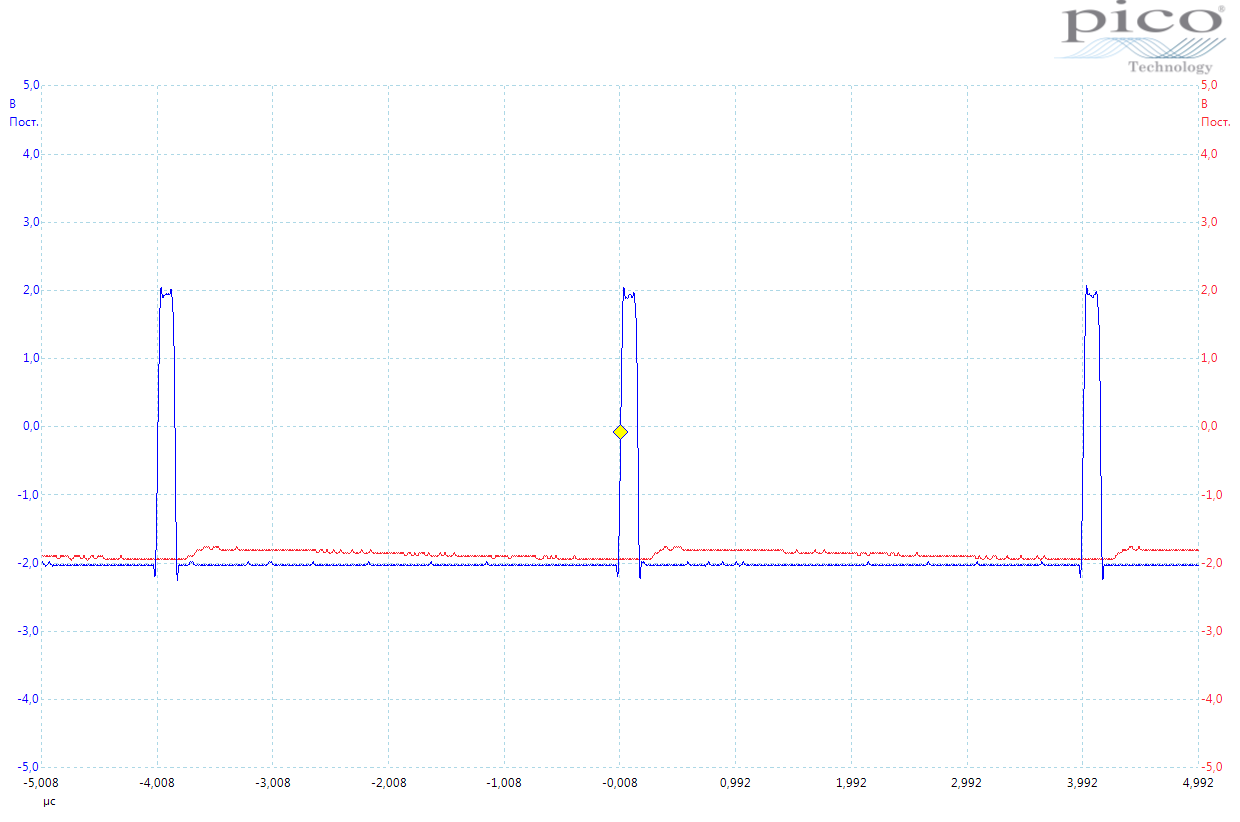
\includegraphics[width=0.9\textwidth]{pictures/27/4_150.png}
	\caption{\textit{Спектр сигнала на выходе RC-цепочки при $T = 4$ мкс, $\tau = 150$ нс}}
	\label{pic:signal-3}
\end{figure}
\FloatBarrier

\clearpage

\begin{enumerate}[resume]
    \item При фиксированном $T = 3$ мкс и $\tau = 250$ нс измерим отношение соответствующих гармоник фильтрованного и исходного сигнала $K_n = a^\text{ф}_n / a^0_n$. Результаты измерений запишем в таблицу \ref{table:6}.
\end{enumerate}

\FloatBarrier
\begin{table}[!ht]
    \centering
    \caption{\textit{Измерение отношения амплитуд фильтрованного и исходного сигнала}}
    \begin{tabular}{|l|l|l|l|l|}
        \hline
        $n$ & $n \nu_0$, кГц & $a^\text{ф}_n$, мВ & $a^0_n$, мВ & $K_n$  \\ \hline
        1 & 333 & 153,7 & 461,1 & 0.333 \\ \hline
        2 & 667 & 78,42 & 439,1 & 0.179 \\ \hline
        3 & 1000 & 51,76 & 414,1 & 0.125 \\ \hline
        4 & 1333 & 25,09 & 379,5 & 0.066 \\ \hline
        5 & 1667 & 25,09 & 334,1 & 0.075 \\ \hline
        6 & 2000 & 20,39 & 291,7 & 0.070 \\ \hline
        7 & 2333 & 10,98 & 244,7 & 0.045 \\ \hline
    \end{tabular}
	\label{table:6}
\end{table}
\FloatBarrier

\begin{enumerate}[resume]
    \item Построим график зависимости $K(\nu), \nu = n \nu_0$, $\nu_0 = 333$ кГц. График изобразим на рис. \ref{graph:4}.
\end{enumerate}

\FloatBarrier
\begin{figure}[!ht]
        \centering
	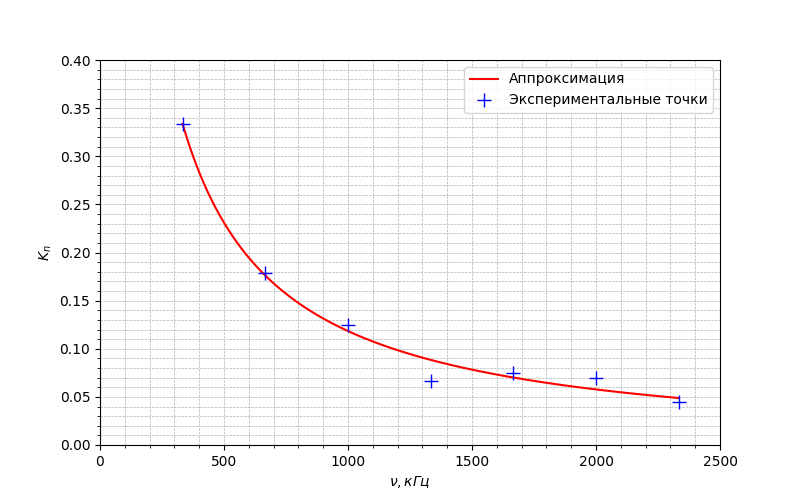
\includegraphics[width=1.0\textwidth]{pictures/graph-29.png}
	\caption{\textit{График зависимости $K(\nu)$}}
	\label{graph:4}
\end{figure}
\FloatBarrier


\end{document}